\section{Introduction}

Crop prediction systems increasingly turn environmental and management data into yield forecasts, suitability scores and crop rankings \citep{liakos2018machine,vanklompenburg2020crop}. These outputs are useful summaries, but they do not answer the operational question of how much land to assign to each crop. Acreage decisions must trade expected returns against land availability, budgets, rotations, contracts and joint downside exposure. Treating the highest-ranked crop as the crop that should receive the most land therefore crosses an unexamined boundary from ordinal prediction to cardinal prescription.

Crop planning research has long represented land use as a constrained portfolio problem. Models incorporate resource constraints, stochastic prices and yields, rotations, robustness and downside risk \citep{filippi2017mixed,boyabatli2019crop,benini2023crop,randall2022robust,randall2024systematic}. In parallel, prescriptive analytics and decision-focused learning show that predictive accuracy and downstream decision quality are distinct evaluation targets \citep{bertsimas2020predictive,elmachtoub2022smart,wilder2019melding,mandi2023decision}. Yet a basic interpretive question remains: what, exactly, can be inferred when a recommendation ranking and an observed or optimized allocation disagree?

This question is difficult for three reasons. First, a ranking is unchanged by every strictly increasing transformation of its scores, whereas proportional allocations are not. Second, constrained optimization may have multiple optimal solutions, so a reversal can hold for one selected optimizer, at least one optimizer or every optimizer. Third, dependence affects portfolio losses through the complete joint distribution; a scalar tail-dependence coefficient cannot generally order conditional losses or acreage \citep{demarta2005tcopula,ansari2024dependence}. These distinctions invalidate simple equivalences between ranks, marginal optimality conditions and acreage levels.

Here we retain the teacher Draft's integrated multi-crop architecture but repair its claims around a set-valued identification framework (Fig.~\ref{fig:concept}). We formulate expected-profit maximization over a polyhedral operational set under loss-CVaR, using the atom-safe representation of \citet{rockafellar2000optimization,rockafellar2002conditional}. We define possible, universal, selected, strong and top-rank reversal; derive a complete subgradient Karush--Kuhn--Tucker characterization; and describe dependence effects through restricted distributional ordering and crossing sets rather than a universal unique threshold. Information and flexibility are retained through actionability and weak feasible-set monotonicity, not asserted to be strictly complementary in general.

The empirical analysis then asks a deliberately narrower question: how often do transparent rankings and observed planted-acreage ranks disagree in an official complete-case state sample? Across \NStateYears{} three-crop state-years in \NStates{} states, operating-margin top ranks disagree with acreage ranks in \OperatingTopCount{} cases. This pattern is definition-sensitive, with top-rank discordance ranging from \DefinitionMinRate\% to \DefinitionMaxRate\%, and it disappears in the retained national comparison. These are descriptive facts, not evidence that observed acreage solves our stochastic programme or that CVaR, copulas or any single constraint caused the disagreement.

The paper contributes a disciplined bridge between rankings and allocations. It establishes what ordinal information cannot identify, supplies solution-set-aware reversal definitions, integrates operational and downside-risk constraints in a reproducible model, and demonstrates how empirical discordance can be reported without assigning an unobserved mechanism. The simulation component is also informative by failure: although all primary solves and numerical replays pass, none of the predeclared convergence rows meets the joint precision rule. We therefore quarantine its substantive patterns to the Supplementary Information. This separation of theorem, simulation, empirical and boundary evidence is central to the study.

\begin{figure}[t]
\centering
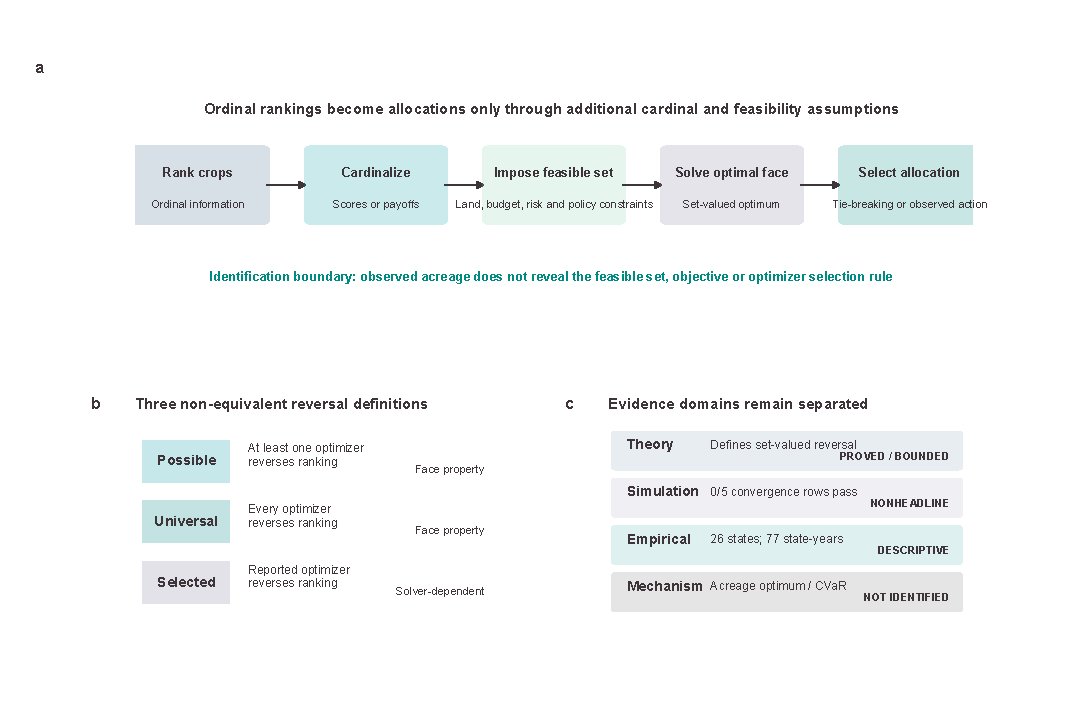
\includegraphics[width=\textwidth]{../figures/main/Figure1.pdf}
\caption{From ordinal crop rankings to set-valued allocation claims. The flow distinguishes additional cardinal and feasibility assumptions, three non-equivalent reversal definitions, and the boundaries between theorem, simulation and empirical evidence.}
\label{fig:concept}
\end{figure}
